\chapter{State-of-art solutions}

	Only one open source application was found suitable for study, Siestta ,  nevertheless there are a lot of educational software (Sixa
	\cite{Sixa}, Unisoft \cite{Unisoft} ) but they are privative, Microsoft Windows freeware or both (SAS acad�mico). 


\section{Siestta}


Technically Siestta\cite{Siestta} is an GPL'ed 1990's style PHP-based web application with Ajax, an interactive editor, fckeditor and fpdf to generate reports.

\begin{figure}
    \begin{center}
        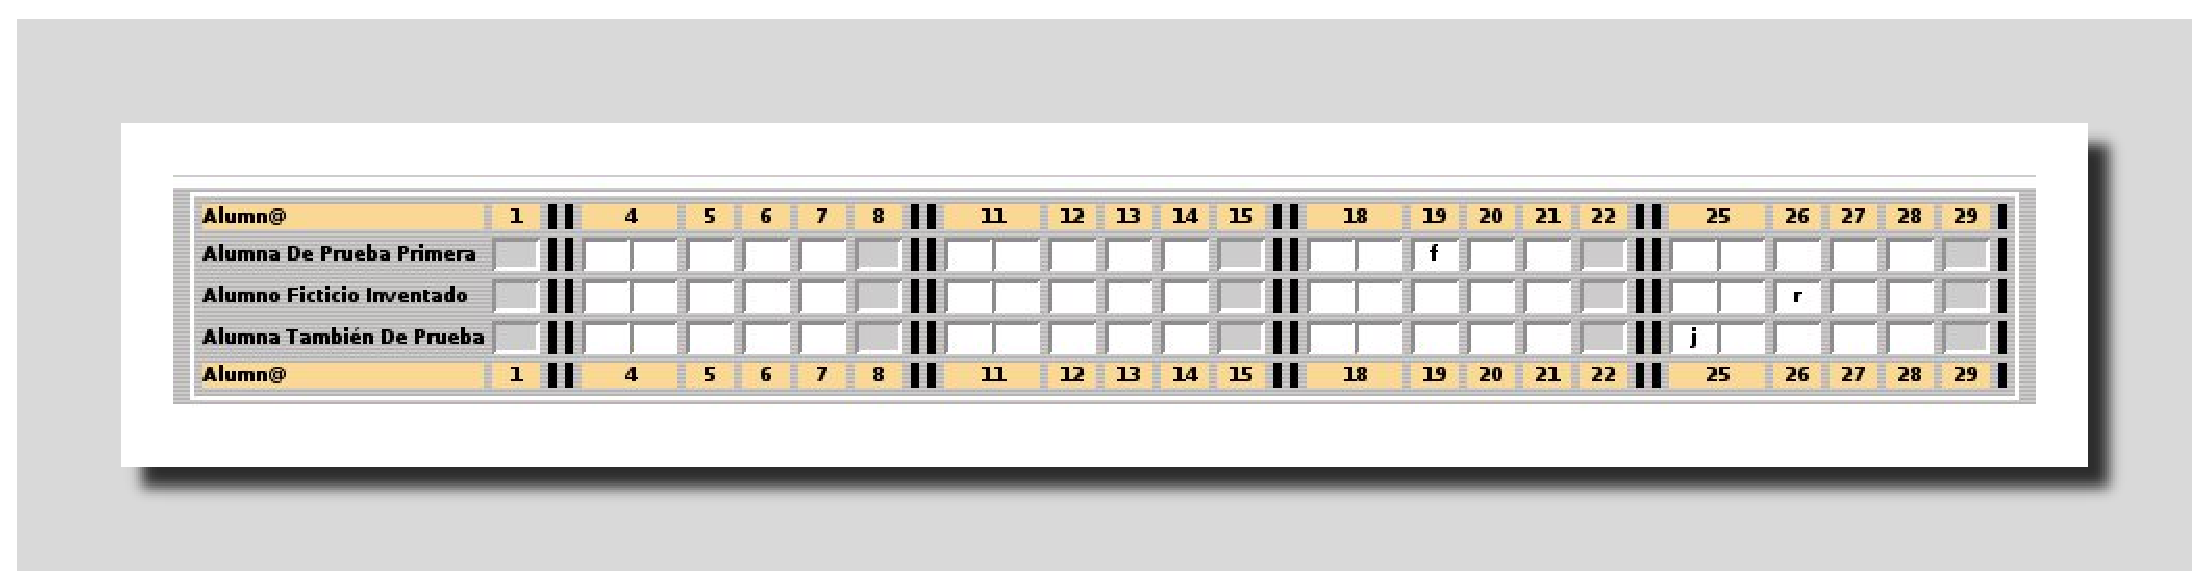
\includegraphics[width=\textwidth]{siestta1.eps}
        \caption{Siestta Attendance Page}
        \label{fig:siestta1}
    \end{center}
\end{figure}

From user point-of-view there are online documentation. This application includes management of students, attendance, marks, tasks, incidents, general queries, letters to parents, interviews with parents, messages, appointments, exams and more.

Several screenshots were taken and their structure will be reused in current application, specially attendance page \ref{fig:siestta1}, and daily schedule \ref{fig:siestta2}.

\begin{figure}
    \begin{center}
        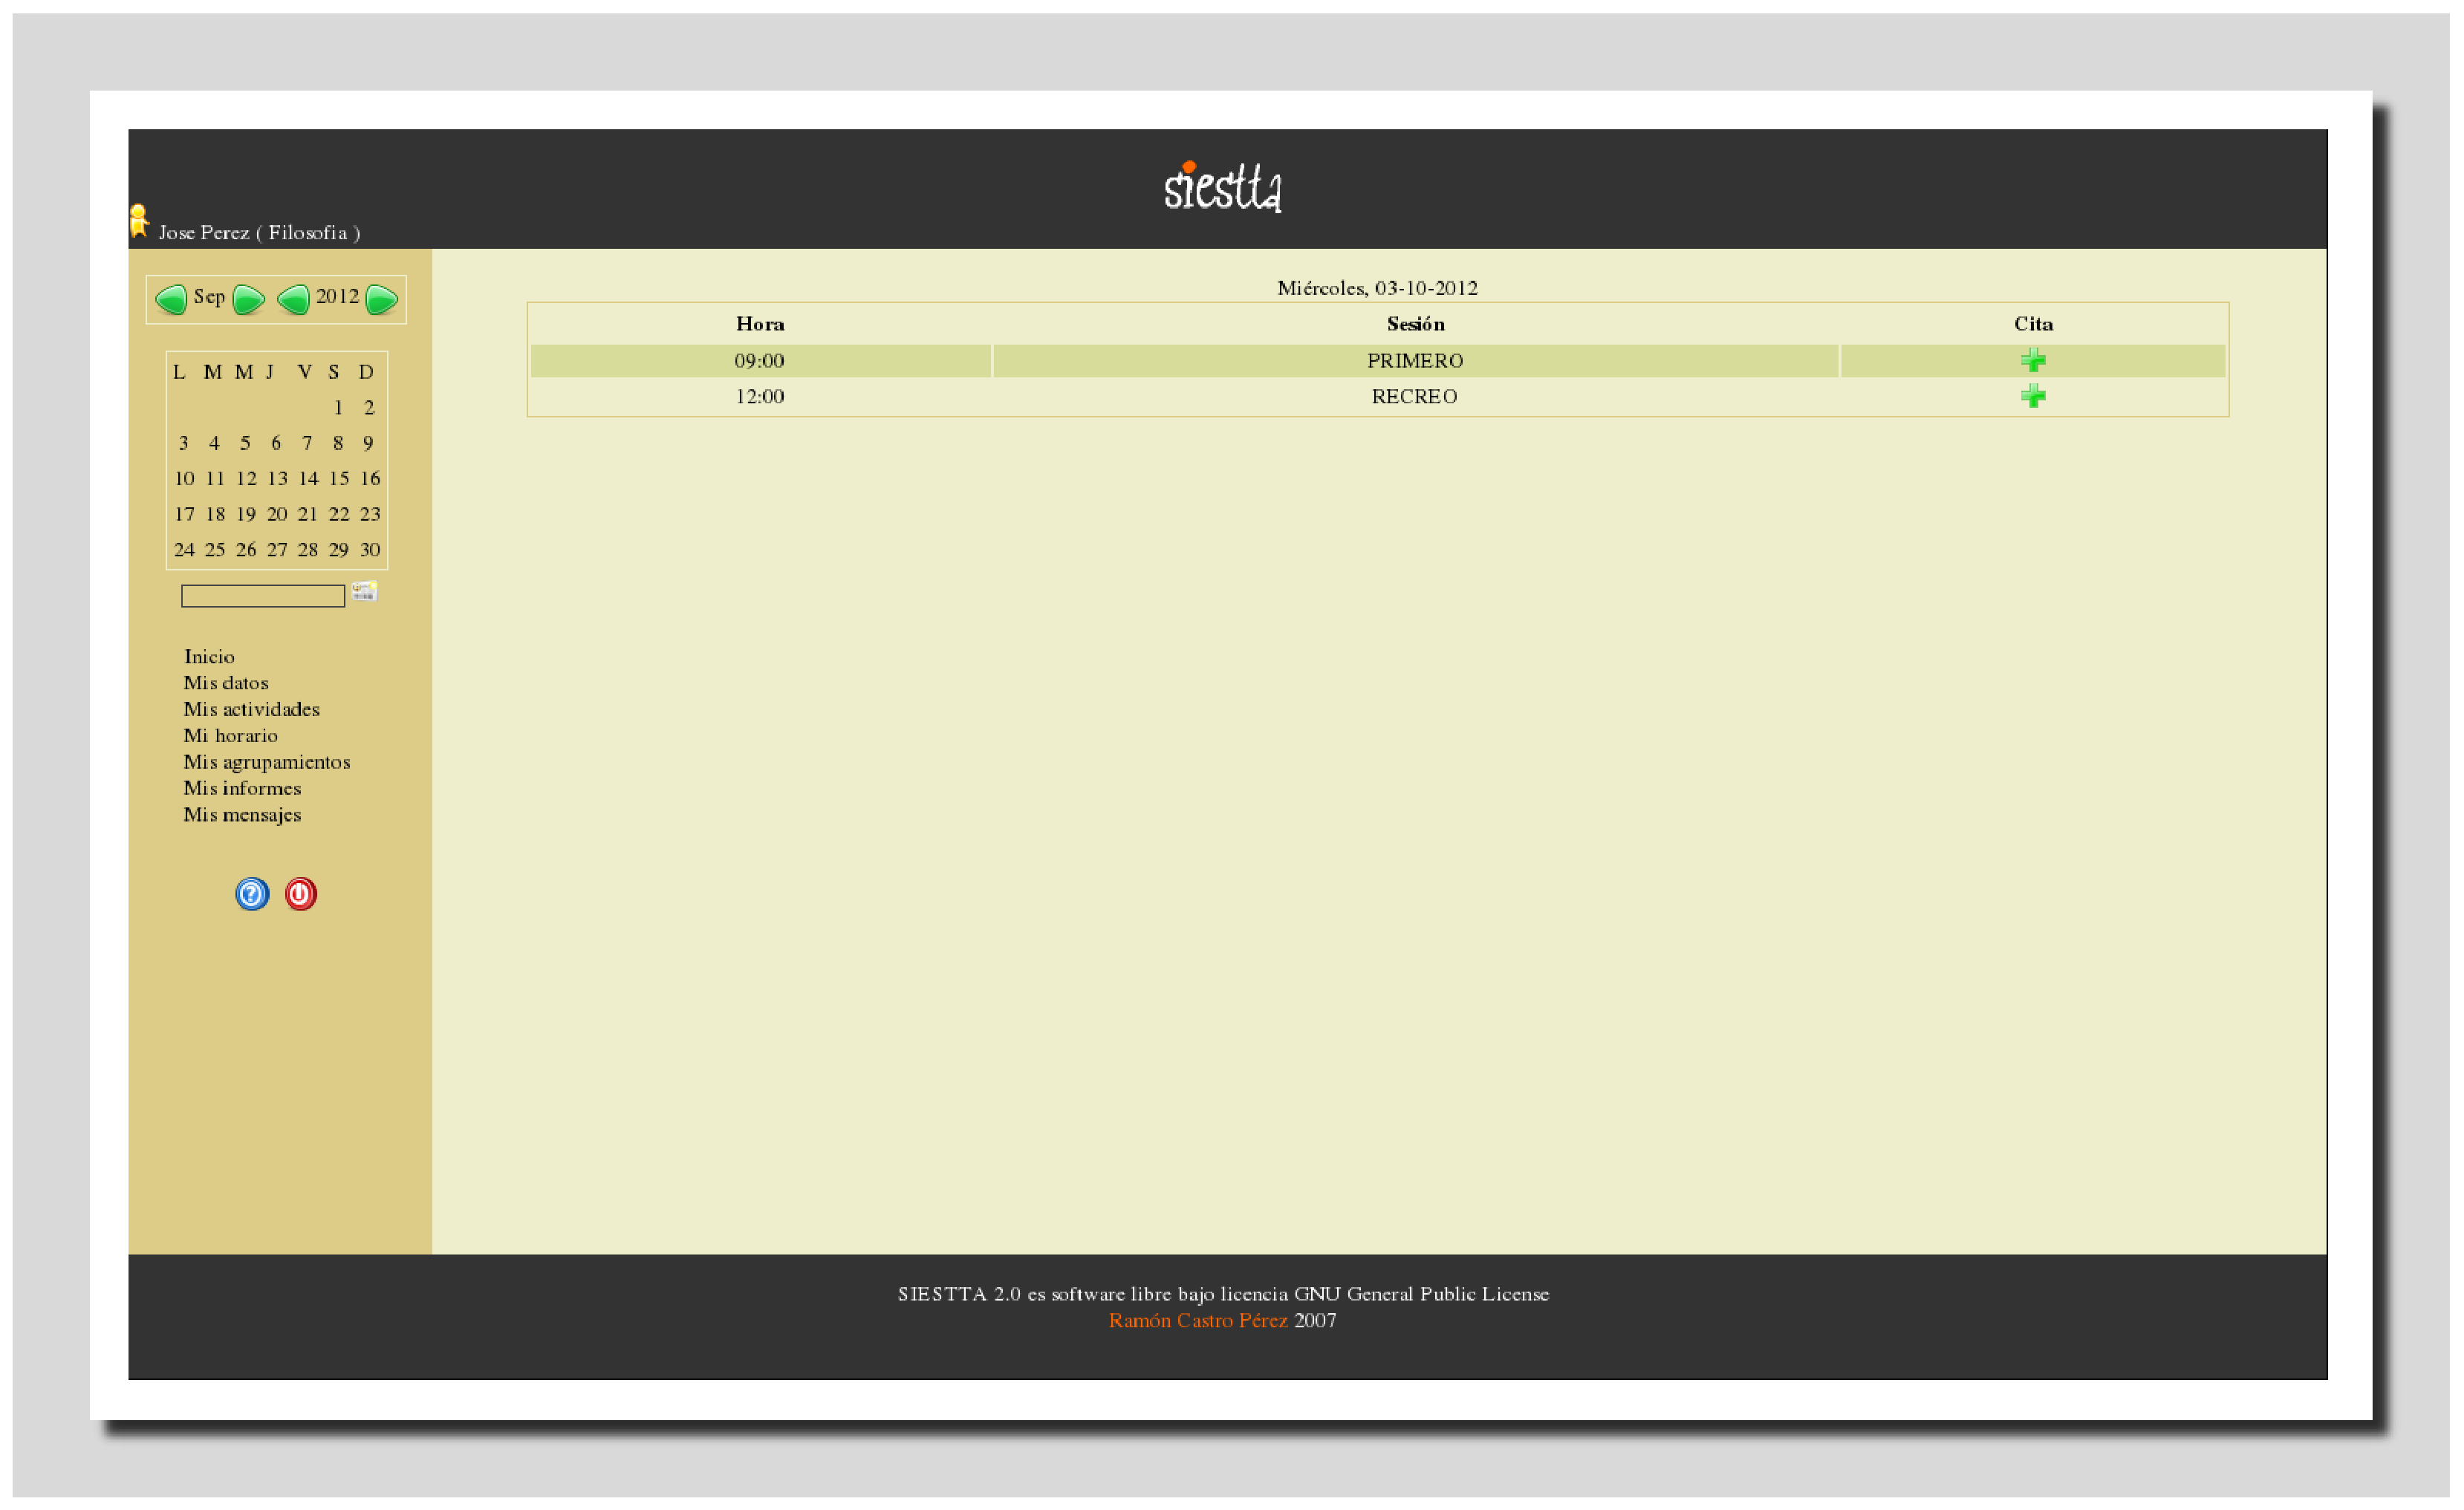
\includegraphics[width=\textwidth]{siestta2.eps}
        \caption{Siestta Main Page}
        \label{fig:siestta2}
    \end{center}
\end{figure}


This application are also available for PDAs, it could be a valid solution but it is server-side with outdated technologies. 
Data structure from Siestta is standard and fully functional, and it will be partially reused by EduXes.\ref{fig:siestta4}.

\begin{figure}
    \begin{center}
        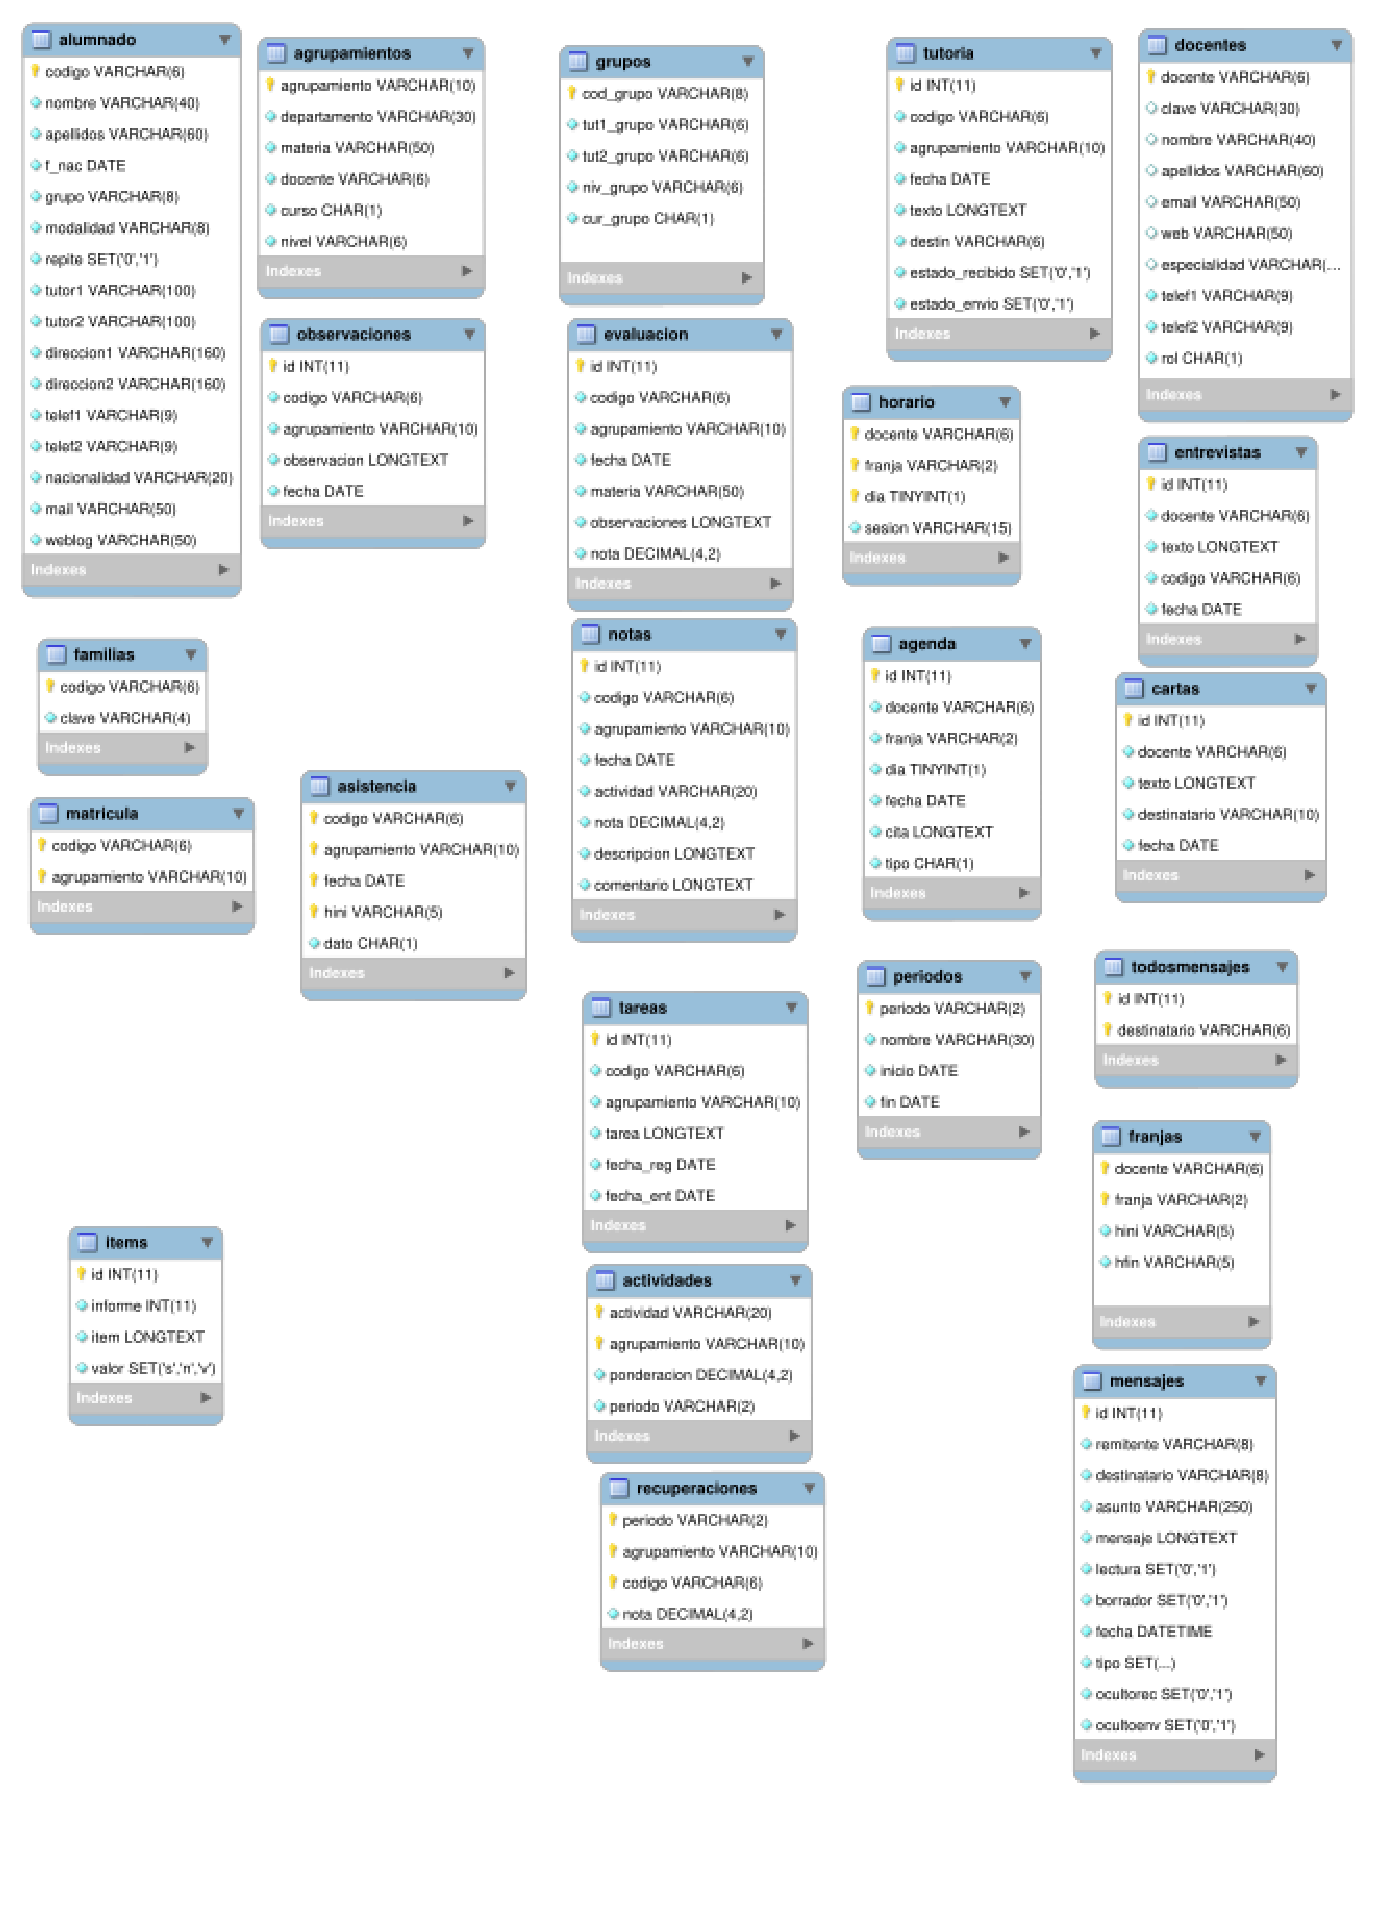
\includegraphics[width=\textwidth]{siestta_sql.eps}
        \caption{Siestta SQL}
        \label{fig:siestta4}
    \end{center}
\end{figure}


Source code are also shown: calendario.php. It shows us a PHP application which uses sessions variables and is not Model-View-Controller oriented.

\begin{bclogo}[couleur=blue!30,arrondi=0.1,ombre=true ] 
{Sample Siestta code: calendario.php}        
        \begin{verbatim}
<?php 
session_start(); 
require('config.php'); 
require('idioma/'.$idioma.''); 
include('funciones_calendario.php'); 
$docente = $_SESSION['usuario_sesion']; 
//recogemos variables 
$mes_actual = $_POST['mes']; 
$anyo_actual = $_POST['anyo']; 
if($mes_actual || $anyo_actual) { 
	include('funciones.php');
	conecta(); 
	}
//si es la primera vez que entramos, cargamos la fecha actual 
if(!isset($mes_actual)) $mes_actual = date('m'); 
if(!isset($anyo_actual)) $anyo_actual = date('Y'); 
//presentamos ahora el calendario del mes actual o cargado 
//tabla con nombre mes y a�o y las flechas para navegar 
echo ' 
<br /> 
<table class="tablacentrada_i"> 
<tr> 
<td> 
<a href="#" onclick="navegaMes(\''.$mes_actual
.'\',\''.$anyo_actual.'\',\'menos\')" title="'.$id_anterior
.'"><img src="imgs/anterior_peq.png" class="alin_bajo" alt="'
.$id_anterior.'" /></a> 
'; 
\end{verbatim}  
\end{bclogo}



\section{Sixa}
Although not GPL'ed, and there are no source code available, several design ideas could be considered: for main page \ref{fig:sixa1},
schedule page \ref{fig:sixa2} and reports page \ref{fig:sixa3}.
\begin{figure}
    \begin{center}
        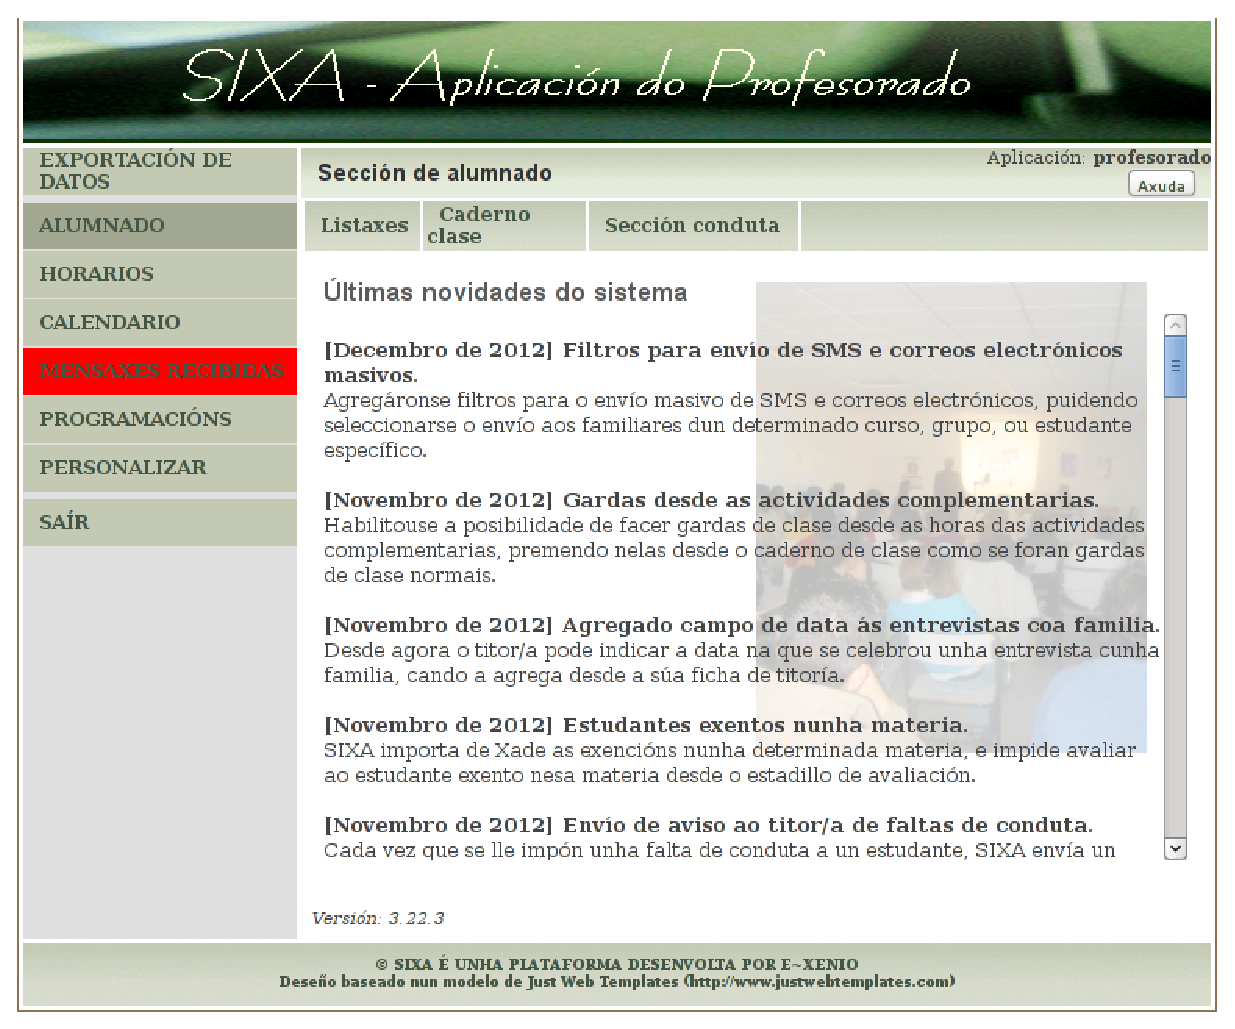
\includegraphics[width=\textwidth]{sixa_1.eps}
        \caption{Sixa Main Page}
        \label{fig:sixa1}
    \end{center}
\end{figure}

\begin{figure}
    \begin{center}
        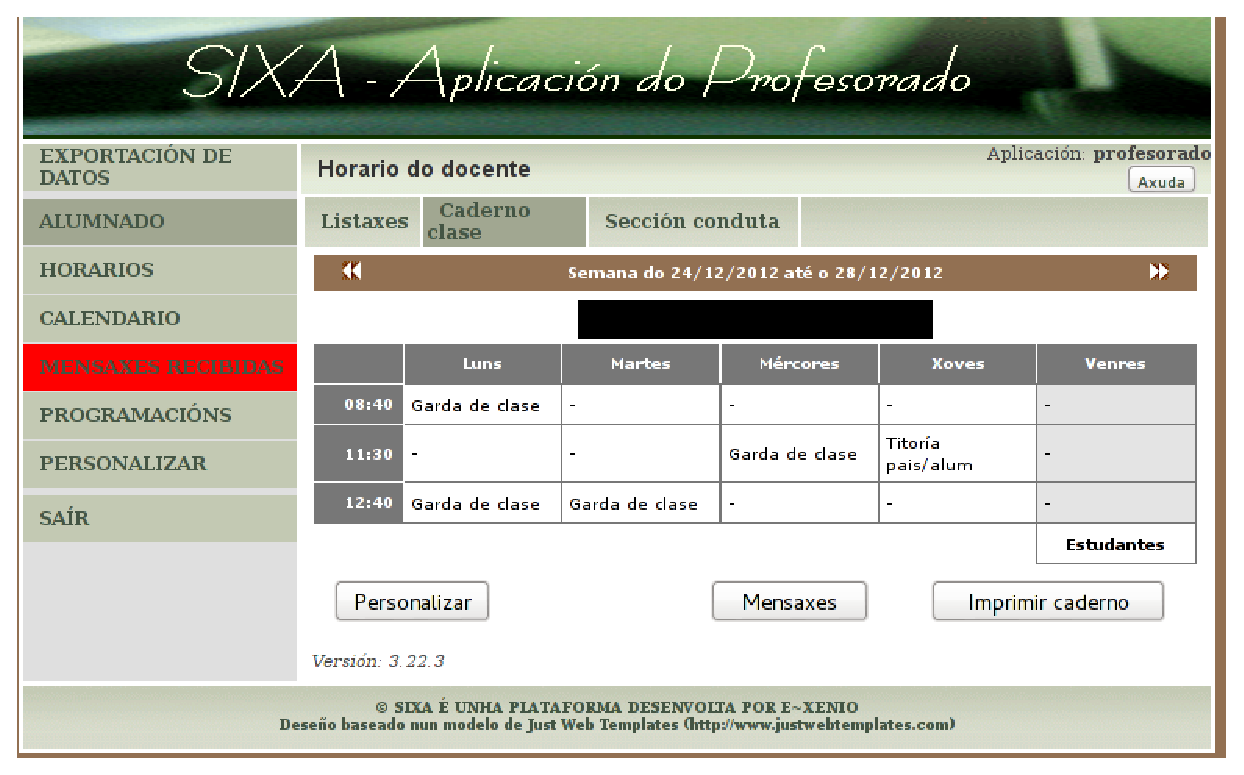
\includegraphics[width=\textwidth]{sixa_2.eps}
        \caption{Sixa Schedule Page}
        \label{fig:sixa2}
    \end{center}
\end{figure}

\begin{figure}
    \begin{center}
        \includegraphics[width=\textwidth]{sixa_3.eps}
        \caption{Sixa Reports Page}
        \label{fig:sixa3}
    \end{center}
\end{figure}
 It has a PDA version (not shown), and it Xade data import capable. Also has a long list of features \cite{Sixa}.


\section{Android applications}
 Several Android applications are listed below, in a short list:

\subsection{Grade Book}
\begin{itemize}
    \item {Name}: Grade Book \cite{Android:Gradebook}
    \item {Description}:Now teachers can manage their students grades directly on their Android device!
    \item {Key Features}:
    \subitem Sync with Google Spreadsheets
    \item {Updated}:July 7, 2011.
    \item {Price }:4 \geneuro
    \item {Screenshot}: \ref{fig:Grade Book}  
\end{itemize}

     
\begin{figure}
    \begin{center}
        \includegraphics[scale=0.5]{grade_book01.jpg}
        \caption{Grade Book}
        \label{fig:Grade Book}
    \end{center}
\end{figure}

\subsection{Attendance}

\begin{itemize}
    \item {Name}: Attendance \cite{Android:Attendance}
    \item {Description}:Attendance control sync with Google Spreadsheet.
    \item {Key Features}: attendance.
    \item {Updated}:January 13, 2012.
    \item {Price }: Free
        \item {Screenshot}: \ref{fig: Android Attendance}
\end{itemize}


\begin{figure}
    \begin{center}
        \includegraphics[scale=0.5]{attendance01.png}
        \caption{Attendance}
        \label{fig:Android Attendance}
    \end{center}
\end{figure}




\subsection{Teacher Organizer }
\begin{itemize}
    \item {Name}: Teacher Organizer  \cite{Android:teacherorganizer}
    \item {Description}:Gradebook and attendance, notes, schedule a teacher (high school teacher).
    \item {Key Features}:
    Unified information resource teacher developed within diploma projects.
    \item {Updated}:  December 26, 2012.
    \item {Price }: Free.
      \item {Screenshot}: \ref{fig:TeacherOrganizer}  
\end{itemize}
 It has a drawback: its web page is in Russian, and it is not translated. This application seems to be very professional. There is no code
 avaliable.

\begin{figure}
    \begin{center}
        \includegraphics[scale=0.5]{teacher_organizer01.jpg}
        \caption{Teacher Organizer}
        \label{fig:TeacherOrganizer}
    \end{center}
\end{figure}


\subsection{Teacher Aide  }

\begin{itemize}
    \item {Name}: Teacher Aide  \cite{Android:TeacherAide}.
    \item {Description}:The app allows teachers to take attendance and record grades on their phone or tablet.
    \item {Key Features}: Import - export data via CSV. Print via a Google service.
    \item {Updated}: 26 December 2012.
    \item {Price }: Free (Limited number of students).
    \item {Screenshot}: \ref{fig:TeacherAide}  
\end{itemize}

Excellent but not open source or even free.

\begin{figure}
    \begin{center}
        \includegraphics[scale=0.5]{TeacherAideProLite01.jpg}
        \caption{Teacher Aide}
        \label{fig:TeacherAide}
    \end{center}
\end{figure}


